\section{Results}

Two sets of data were taken, and are examined here in terms of the accuracy of
their produced models and the possible causes of error in the reconstruction
process. The first set of photographs were taken at Long Ashton Farm outside
Bristol, and the second set were taken at the Avon Gorge in Bristol.

\subsection{Long Ashton}

For this data set, a hexacopter was used to gather a total of 63 aerial images.
The time interval technique was used to take the photos, and the time offset
method used to geotag the resulting photos.

\subsubsection{Without GCPs}
\label{sec:results/long-ashton/no-gcp}

Firstly, the reconstruction was run without the Ground Control Points input, and
without any photographic alignment optimisation. The resulting orthophoto is
shown in Figure \ref{img:long-ashton/no-gcps/orthophoto}, while the DEM is shown
in Figure \ref{img:long-ashton/no-gcps/dem} and the photographic overlap is shown
in Figure \ref{img:long-ashton/no-gcps/overlap}. The produced model is available
to view interactively online at
\url{https://sketchfab.com/models/ad8a1d9f8c324eb592a9e4beabc5a51e}.

\begin{figure}
    \centering
    \begin{subfigure}[b]{0.3\textwidth}
        \includegraphics[width=\textwidth]{LongAshton/NoGCPs/Orthophoto}
        \caption{The generated orthophoto for the Long Ashton data set, without
        GCPs input.}
        \label{img:long-ashton/no-gcps/orthophoto}
    \end{subfigure}
    \begin{subfigure}[b]{0.3\textwidth}
        \includegraphics[width=\textwidth]{LongAshton/NoGCPs/DEM}
        \caption{The generated DEM for the Long Ashton data set, without GCPs
        input.}
        \label{img:long-ashton/no-gcps/dem}
    \end{subfigure}
    \begin{subfigure}[b]{0.3\textwidth}
        \includegraphics[width=\textwidth]{LongAshton/NoGCPs/Overlap}
        \caption{The calculated photographic overlap achieved in the Long Ashton
        photo dataset.}
        \label{img:long-ashton/no-gcps/overlap}
    \end{subfigure}
    \caption{The data produced by PhotoScan from the Long Ashton aerial imagery,
    without factoring in GCPs.}
    \label{img:long-ashton/no-gcps}
\end{figure}

Clearly, the orthophoto shows that the 63 photos were sufficient to build a
model of the topography of the area. However, the Digital Elevation Model shows
that the photogrammetric reconstruction interpreted the topography as on a
significant tilt head from the car park up to the building. We hypothesise that
this tilt is due to the lack of GCPs to correct for such systematic errors. This
is discussed with reference to the model produced \textit{with} GCPs in Section
\ref{sec:results/long-ashton/wth-gcps} and also with reference to the Avon Gorge
reconstruction in Section \ref{sec:results/avon-gorge}.

DEM and model accuracy.

Good overlap.

\subsubsection{With GCPs}
\label{sec:results/long-ashton/wth-gcps}

The reconstruction was then rerun with a limited number of Ground Control Points
input. These GCPs were taken using distinguishable features from the landscape
and their geolocation found from Google Earth to test the effect they would have
on the resulting model and DEM. The first DEM was taken as the centre of a pond,
the second the corner of a fence and the third

\begin{figure}
    \centering
    \begin{subfigure}[b]{0.3\textwidth}
        \includegraphics[width=\textwidth]{LongAshton/WithGCPs/Orthophoto}
        \caption{The generated orthophoto for the Long Ashton data set, with 3
        GCPs input.}
        \label{img:long-ashton/with-gcps/orthophoto}
    \end{subfigure}
    \begin{subfigure}[b]{0.3\textwidth}
        \includegraphics[width=\textwidth]{LongAshton/WithGCPs/DEM}
        \caption{The generated DEM for the Long Ashton data set, with 3 GCPs
        input.}
        \label{img:long-ashton/with-gcps/dem}
    \end{subfigure}
    \begin{subfigure}[b]{0.3\textwidth}
        \includegraphics[width=\textwidth]{LongAshton/WithGCPs/Overlap}
        \caption{The calculated photographic overlap achieved in the Long Ashton
        photo dataset with 3 GCPs.}
        \label{img:long-ashton/with-gcps/overlap}
    \end{subfigure}
    \caption{The data produced by PhotoScan from the Long Ashton aerial imagery,
    with 3 GCPs input.}
    \label{img:long-ashton/with-gcps}
\end{figure}

\subsection{Avon Gorge}
\label{sec:results/avon-gorge}

This model was reconstructed from two passes of 87 and 61 photos. As before, the
time interval with time offset techniques were used for taking photos and
geotagging the photos, respectively. The photos were taken by attaching the
camera to the quadcopter and 

\subsubsection{Without GCPs}

\begin{figure}
    \centering
    \begin{subfigure}[b]{0.3\textwidth}
        \includegraphics[width=\textwidth]{AvonGorge/NoGCPs/Orthophoto}
        \caption{The generated orthophoto for the Avon Gorge data set, no 14
        GCPs input.}
        \label{img:avon-gorge/no-gcps/orthophoto}
    \end{subfigure}
    \begin{subfigure}[b]{0.3\textwidth}
        \includegraphics[width=\textwidth]{AvonGorge/NoGCPs/DEM}
        \caption{The generated DEM for the Avon Gorge data set, no 14 GCPs
        input.}
        \label{img:avon-gorge/no-gcps/dem}
    \end{subfigure}
    \begin{subfigure}[b]{0.3\textwidth}
        \includegraphics[width=\textwidth]{AvonGorge/NoGCPs/Overlap}
        \caption{The calculated photographic overlap achieved in the Avon Gorge
        photo dataset no 14 GCPs.}
        \label{img:avon-gorge/no-gcps/overlap}
    \end{subfigure}
    \caption{The data produced by PhotoScan from the Avon Gorge horizontal
    imagery, no 14 GCPs input.}
    \label{img:avon-gorge/no-gcps}
\end{figure}

\subsubsection{With GCPs}

\begin{figure}
    \centering
    \begin{subfigure}[b]{0.3\textwidth}
        \includegraphics[width=\textwidth]{AvonGorge/WithGCPs/Orthophoto}
        \caption{The generated orthophoto for the Avon Gorge data set, with 14
        GCPs input.}
        \label{img:avon-gorge/with-gcps/orthophoto}
    \end{subfigure}
    \begin{subfigure}[b]{0.3\textwidth}
        \includegraphics[width=\textwidth]{AvonGorge/WithGCPs/DEM}
        \caption{The generated DEM for the Avon Gorge data set, with 14 GCPs
        input.}
        \label{img:avon-gorge/with-gcps/dem}
    \end{subfigure}
    \begin{subfigure}[b]{0.3\textwidth}
        \includegraphics[width=\textwidth]{AvonGorge/WithGCPs/Overlap}
        \caption{The calculated photographic overlap achieved in the Avon Gorge
        photo dataset with 14 GCPs.}
        \label{img:avon-gorge/with-gcps/overlap}
    \end{subfigure}
    \caption{The data produced by PhotoScan from the Avon Gorge horizontal
    imagery, with 14 GCPs input.}
    \label{img:avon-gorge/with-gcps}
\end{figure}

\subsection{Ground Control Point Accuracy}

Which GCPs produced the biggest errors and why. Sources of stated errors in
PhotoScan generated report.

\subsection{Model and DEM Analysis}

\begin{itemize}

    \item PhotoScan calculated meters per pixel.

    \item Error - find out where PhotoScan calculates this from!

    \item Photographics overlap

\end{itemize}
